\documentclass[../main.tex]{subfiles}
\graphicspath{{\subfix{../img/}}}
\begin{document}

\newpage
\section{Lösungskonzept}

In diesem Kapitel wird das gewählte Lösungskonzept ''Simpel'' (siehe Anhang \ref{loesungsvariante_Simpel}) näher erläutert. Bei diesem Konzept liegt der Schwerpunkt auf der Suche nach einer möglichst einfachen Lösung, da ein einfach konstruiertes System in der Regel robuster im Einsatz ist. Im folgenden Text wird für jede Teilfunktion die einfachste Lösung erarbeitet und beschrieben.

\subsection{Ablauf}

Im Ablaufdiagramm (Abbildung \ref{img:ablaufdiagramm}) wird der Ablauf des Roboters von Start bis Ziel übersichtlich aufgezeigt.

\begin{figure}[H]
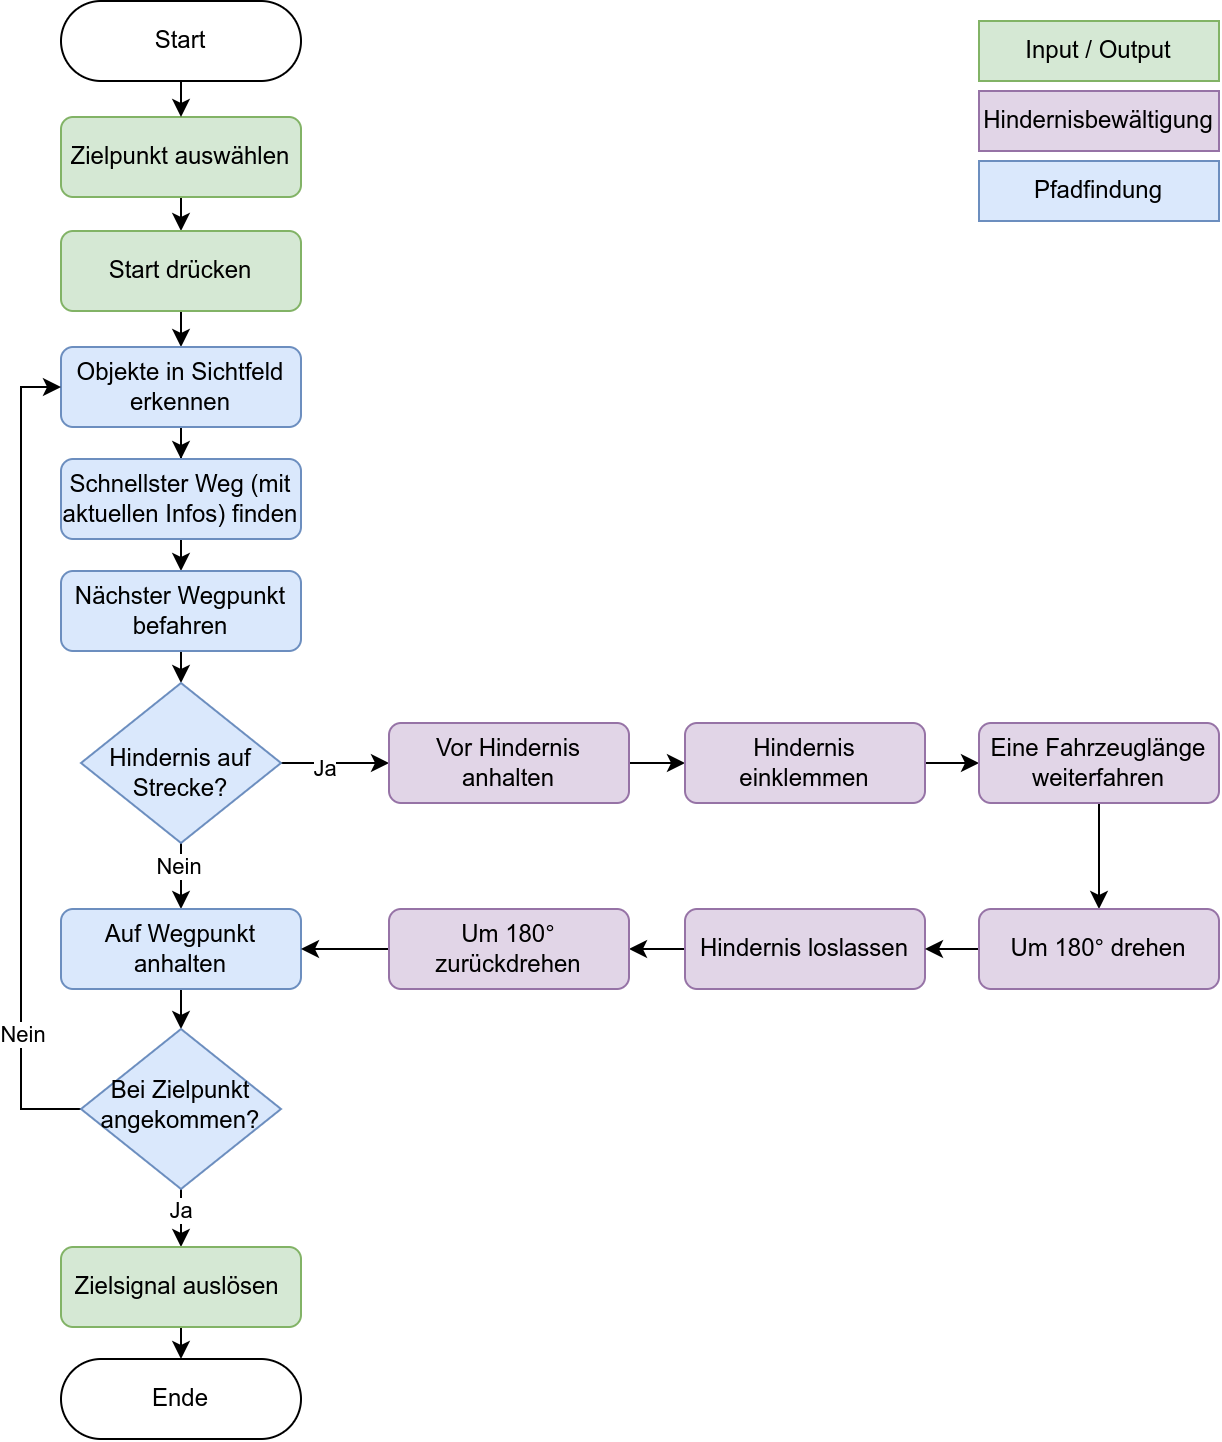
\includegraphics[width=\textwidth]{img/lösungskonzpet/Ablaufdiagramm.png}
\caption{Ablaufdiagramm}
\label{img:ablaufdiagramm}
\end{figure}

\subsection{Fortbewegung}

Die Fortbewegung wird nach dem Prinzip Roomba realisiert. Wie der Name schon erahnen lässt, handelt es sich dabei um ein ähnliches System, wie wir es von Staubsauger-Robotern kennen. Das Prinzip besteht aus zwei einzeln angetriebenen Rädern und einem Stützelement. Die angetriebenen Räder können unabhängig in beide Drehrichtungen drehen, wodurch ein Wenden an Ort und Stelle ermöglicht wird.

\subsection{Ersatz Rotation}    % Gibt es ein besseren Teilfunktion beschrieb für das???



\subsection{Fahrantrieb}
Als Fahrantriebe wurden zwei DC-Getriebemotoren mit Encodern gewählt. DC-Motoren lassen sich einfach mit H-Brücken steuern, wodurch die Drehzahl über ein PWM-Signal geregelt werden kann. Darüber hinaus ermöglicht diese Steuerung die Anpassung der Drehrichtung sowie das Bremsen oder Beschleunigen des Motors. Der Encoder sorgt für einen geschlossenen Regelkreis, sodass die Position des Fahrzeugs jederzeit im Programm berechnet werden kann. Dies ist besonders wichtig für das Anforderungskriterium 4.1, wie in Tabelle \ref{tab:Anforderungsliste} aufgeführt ist. Aus diesem Grund wurde der Schrittmotor ausgeschlossen, da er einen offenen Regelkreis besitzt, bei dem die Gefahr besteht, dass Schritte verloren gehen. Zudem ist die Ansteuerung eines Schrittmotors komplexer als die eines DC-Motors.


\subsection{Hindernisbewältigungsantrieb}



\subsection{Sensorik Positionsabfrage}
Für die Bestimmung der Position des Fahrzeugs wird ein Encoder gewählt, der direkt zusammen mit dem DC-Motor bezogen werden kann. Bei jeder Umdrehung des Motors gibt der Encoder eine bestimmte Anzahl von Impulsen aus. Diese Technologie ist sehr einfach und benötigt lediglich einen Eingang, ohne dass eine I2C-Schnittstelle oder ein weiterer Kommunikationskanal erforderlich ist. Im Gegensatz dazu erfordert ein Beschleunigungssensor einen zusätzlichen Kommunikationskanal. Zudem kumuliert der Fehler eines Beschleunigungssensors mit der Betriebszeit, was zu unzuverlässigen Messwerten führen kann. Aufgrund dieser Nachteile wird der Beschleunigungssensor von vornherein ausgeschlossen. Daher fällt die Wahl auf den Encoder, der aufgrund seiner Einfachheit und Zuverlässigkeit die bevorzugte Lösung darstellt.


\subsection{Bilderkennungssteuerung}



\subsection{Hardware Steuerung}
Zur Auswahl stehen verschiedene Mikrocontroller, darunter der Arduino, der TinyK22 und der ESP32. Im Rahmen dieses Konzepts, das auf Einfachheit setzt, stellt der ESP32 jedoch eine überdimensionierte Lösung dar, da weder WiFi noch Bluetooth in unserem Anwendungsfall benötigt werden. Zudem hat der ESP32 einen höheren Stromverbrauch, der in diesem Kontext nicht gerechtfertigt ist. Aus diesen Gründen scheidet der ESP32 aus.

Der Vorteil des Arduinos liegt in seiner grossen Community und der umfangreichen Online-Hilfe, die zur Verfügung steht. Da jedoch die Elektrotechniker keine Programmiererfahrung in C++ haben und nicht jeder Arduino eine Debugging-Funktion bietet, ist der Arduino nicht die einfachste Lösung.

Der TinyK22 hingegen wurde im Modul Mc Fun ausführlich behandelt. Er bietet eine benutzerfreundliche Programmierumgebung mit integriertem Debugger und wird in C programmiert. Zudem können bei Fragen die Dozenten konsultiert werden, die bereits über umfangreiche Erfahrung mit dem TinyK22 verfügen. In unserem Anwendungsfall stellt der TinyK22 daher die einfachste und effektivste Lösung für die Programmierung dar.


\subsection{Objekterkennung Hindernis}
Das Hindernis wird bereits zu Beginn von der Kamera erkannt. Zur Distanzmessung des Hindernisses wird dann auf einen Ultraschallsensor gewechselt, da dieser ab 3 cm präzise Werte liefert. Zudem ist die Ansteuerung des Ultraschallsensors sehr einfach, da er nur über die Trigger- und Echo-Pins gesteuert wird. Der Time of Flight (TOF) Sensor hingegen wird über eine I2C-Schnittstelle ausgelesen. Im Kapitel Hardware-Test zeigt sich, dass die Messwerte beider Sensoren grundsätzlich ähnlich sind. Der TOF-Sensor hat jedoch den Nachteil von Messfehlern bei direkter Sonneneinstrahlung. Aus diesen Gründen fiel die Wahl auf den Ultraschallsensor.


\subsection{Objekterkennung Pylone}
Die Pylonen werden mit der Kamera erkannt, und zwar mithilfe von Objekterkennungssoftware. Obwohl die Kamera eine komplexere Lösung darstellt, kann der Ultraschallsensor aufgrund der angeschrägten Fläche keinen validen Messwert liefern, ebenso wie der TOF-Sensor. Daher ist die Kamera die zuverlässigste und effektivste Methode, um die Pylonen zu erkennen.


\subsection{Streckenerkennung}
Die Streckenerkennung setzt sich aus zwei Teilen zusammen. Zunächst muss an dem Punkt erkannt werden, in welche Richtung das Fahrzeug weiterfahren soll. Dies wird durch eine Kamera in Verbindung mit einem Raspberry Pi realisiert. Der Raspberry Pi analysiert das Bild und berechnet, um wie viel Grad sich das Fahrzeug drehen muss, um der gewünschten Richtung zu folgen.

Der zweite Teil der Streckenerkennung sorgt dafür, dass das Fahrzeug der Linie folgt. Dies wird durch einen Liniensensor aus Fototransistoren erreicht, der den Unterschied zwischen der Linie und dem Boden erkennen kann. Auf dieser Grundlage steuert der Sensor das Fahrzeug so, dass es konstant auf der Linie bleibt.

\subsubsection{Streckenerkennung Kamera}

TODO: Gian
- Wegpunkt wird mittels Objekterkennung erkannt (siehe ref)
- Linien bei Wegpunkt erkennen
  - Canny Edge Detection (Technologierecherche)
  - Hough Line Transform



\subsection{Punktverifizierung}
Der Punkt wird auf die gleiche Weise wie die Linie mit dem Liniensensor erkannt. Der Liniensensor ist so breit wie der Punkt, was bedeutet, dass, wenn der Liniensensor auf dem Punkt platziert ist, alle Fototransistoren gleichzeitig die Linie erkennen. Dieser Zustand signalisiert, dass das Fahrzeug auf einem Punkt steht.


\subsection{Objekterkennung Software}




\subsection{Wegfindungssoftware}

Um den schnellsten Weg ins Ziel zu finden, wird der Graph in der Software abgespeichert
und der kürzeste Weg mittels Dijkstra Algorithmus berechnet. Sobald neue Informationen der Strecke erkannt werden, wird der Graph entsprechend angepasst und der kürzeste Weg wird anhand der aktuellen Position neu ermittelt.
Ursprünglich haben alle Linien im Graphen eine einheitliche Gewichtung. 

Je nach neu erhaltener Information werden andere Anpassungen am Graphen vorgenommen:
\begin{itemize}
    \item Pylon auf Wegpunkt erkannt: Wegpunkt (Knote) wird aus dem Graphen entfernt
    \item Linie wurde entfernt: Linie (Kante) wird aus dem Graphen entfernt.
    \item Hindernis auf Linie erkannt: Linie (Kante) erhält mehr Gewichtung.
\end{itemize}

\subsection{Energiequelle}
Aus der Technologierecherche hat sich herausgestellt, dass der LiPo-Akku der am besten geeignete Akku im Vergleich zu Li-Ion- und NiMH-Akkus ist. Dies liegt insbesondere an seiner höheren Leistungsdichte, besseren Leistungsabgabe und der Flexibilität in der Formgebung. Weitere Details dazu können im Anhang unter der Sektion Konzeptfindung \ref{subsec:Energiequelle} nachgelesen werden.

\newpage
\subsection{Aufnahme Hindernis}
Wie bereits beschrieben wurde das Greifkonzept "Klemme seitlich" ausgewählt (siehe \ref{loesungsvariante_Simpel}).
Damit dieses erfolgreich umgesetzt werden kann, wurden Dimensionen vom Greifer definiert  sowie ein passendes Konzept für den Mechanismus gefunden. Zusätzlich wurde der hebe Mechanismus und der Greifmechanismus so konstruiert das es mit einem linear Motor angesteuert werden kann.
Die Recherche und Entscheidungen die zu diesen ausgearbeiteten Konzept geführt hat sind im Anhang: \ref{hier muss noch ein Anhang hin} ersichtlich.

%Im anhang sollte das stehehen
%allgemeines Konzept, etc entscheidung aus konzeptfindung
%Entscheidung alles mit einem Motor

\subsubsection{Dimensionen Greifarm}
Wie bereits im Kapitel \ref{a3:Präzision} erwähnt, ist die Präzision, die mechanisch gewonnen werden kann, sehr relevant für dieses Konzept. Damit dies auch funktioniert, wurden die passenden Dimensionen der Klemme eruiert. 

\paragraph{Winkel Verschiebung}
Nach Aufgabenstellung kann das Hindernis bis zu 15° verschoben sein.
In der Abbildung \ref{img:loes_winkel_hinderniss} ist dies bildlich dargestellt.

\begin{figure}[H]
        \centering
        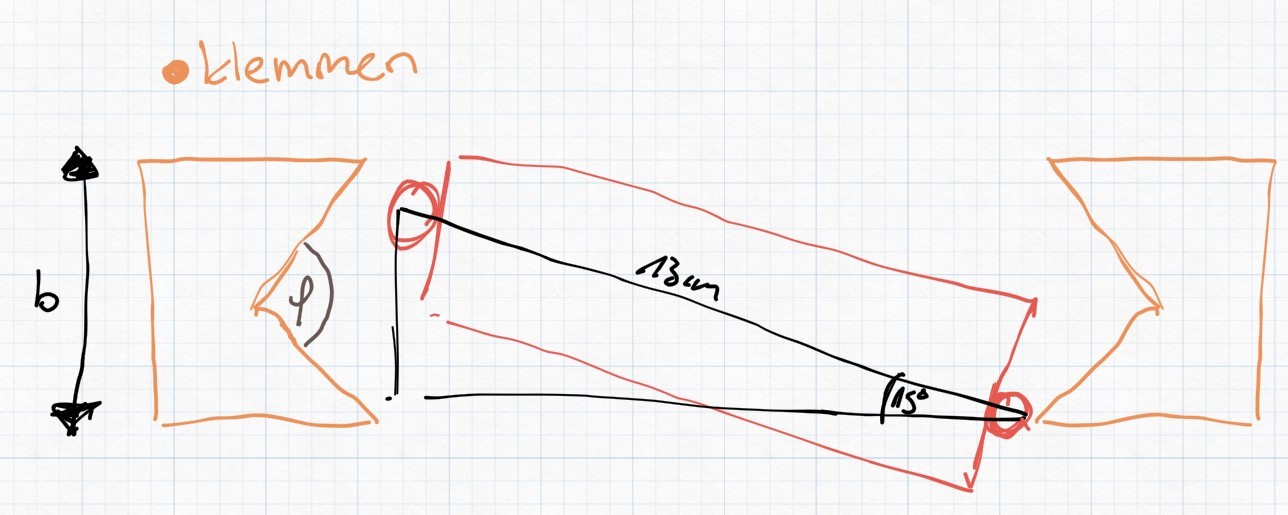
\includegraphics[width=0.48\textwidth]{img/lösungskonzpet/hindernissaufnahme/winkekl_klemmen.jpg}
        \caption[Möglicher Winkel des Hinderniss]{Möglicher Winkel des Hinderniss \footnotemark} 
        \label{img:loes_winkel_hinderniss}
\end{figure}

Damit kann $b$ ausgerechnet werden:

\[
b = 13cm * sin(15) = 3.36cm
\]

Damit genügend Sicherheit hierbei eingerechnet wird, haben wir uns entschieden $b = 4.5cm$ zu machen. Dies wird uns helfen Fehler in der Distanzmessung auszugleichen.

$\varphi$ wurde 90° gewählt, dies ist vorläufig eine Annahme und muss zu einem späteren Zeitpunkt getestet werden.

\paragraph{Abstand der Klemmen}


\newpage
\subsubsection{Funktionalitäten}
Greifen -> Heben -> absetzen -> Loslasasen
korrektur Distanz
Korrektur Winkel
Korrektur Offset

\


\subsection{Rotation / Translation Hindernis}





\end{document}